\section{System Architecture}
\label{sec:arch}

\subsection{Design Principles and Specification}

The AI SOC Analyst Agent is governed by a formal behavioral specification written
in RFC~2119 modal language (MUST, SHOULD, MAY) to ensure auditability across
deployment environments. The specification enforces three invariants: (1) all
tool calls are strictly read-only with no side-effect permissions on production
infrastructure; (2) every investigation verdict is accompanied by a structured
evidence provenance chain; and (3) escalation decisions are made exclusively by the
Evidence Fusion Engine under explicit threshold governance.

\subsection{Eight-Module Functional Architecture}

The system decomposes into eight decoupled functional modules as illustrated
in Fig.~\ref{fig:arch}:

\begin{itemize}
  \item \textbf{\textcircled{1} Alert Queue Interface:} Receives normalized alert
  events from SIEM/XDR systems via a typed JSON schema, validates mandatory fields
  (host ID, timestamp, alert category, severity score), and enqueues validated
  incidents for processing.

  \item \textbf{\textcircled{2} Alert Ingestion and Normalization:} Performs
  schema validation, deduplication within a 15-minute sliding window, and
  feature extraction for downstream classification.

  \item \textbf{\textcircled{3} Planner and Reasoning Agent:} Orchestrates the
  bounded ReAct+RAG control loop (Algorithm~1) with a maximum hop budget
  $B \le 5$ tool invocations per investigation.

  \item \textbf{\textcircled{4} Data Acquisition and Evidence Store:} Executes
  parameterized SQL queries over relational endpoint telemetry tables. All queries
  are pre-approved read-only templates to prevent injection vulnerabilities.

  \item \textbf{\textcircled{5} Analytics Engine:} Computes calibrated GBDT
  posterior probabilities $(P_{\text{TP}}, P_{\text{BP}}, P_{\text{FP}})$ and
  TreeSHAP feature attributions for LLM context injection.

  \item \textbf{\textcircled{6} Domain Knowledge Engine:} Retrieves MITRE ATT\&CK
  STIX~2.1 technique objects and NIST SP~800-61r3 response playbook steps via
  dense vector retrieval over a local embedding index.

  \item \textbf{\textcircled{7} Decision and Evidence Fusion Engine:} Integrates
  GBDT posteriors, LLM reasoning outputs, and retrieved knowledge to compute the
  final fusion probability $P_{\text{fusion}}$, applying the asymmetric escalation
  policy against threshold $\tau_{\text{conf}}$.

  \item \textbf{\textcircled{8} Output and Interaction Module:} Generates structured
  triage reports with evidence provenance, recommended remediation steps, and an
  escalation flag for Tier-2 analyst review.
\end{itemize}

\begin{figure}[t]
\centering
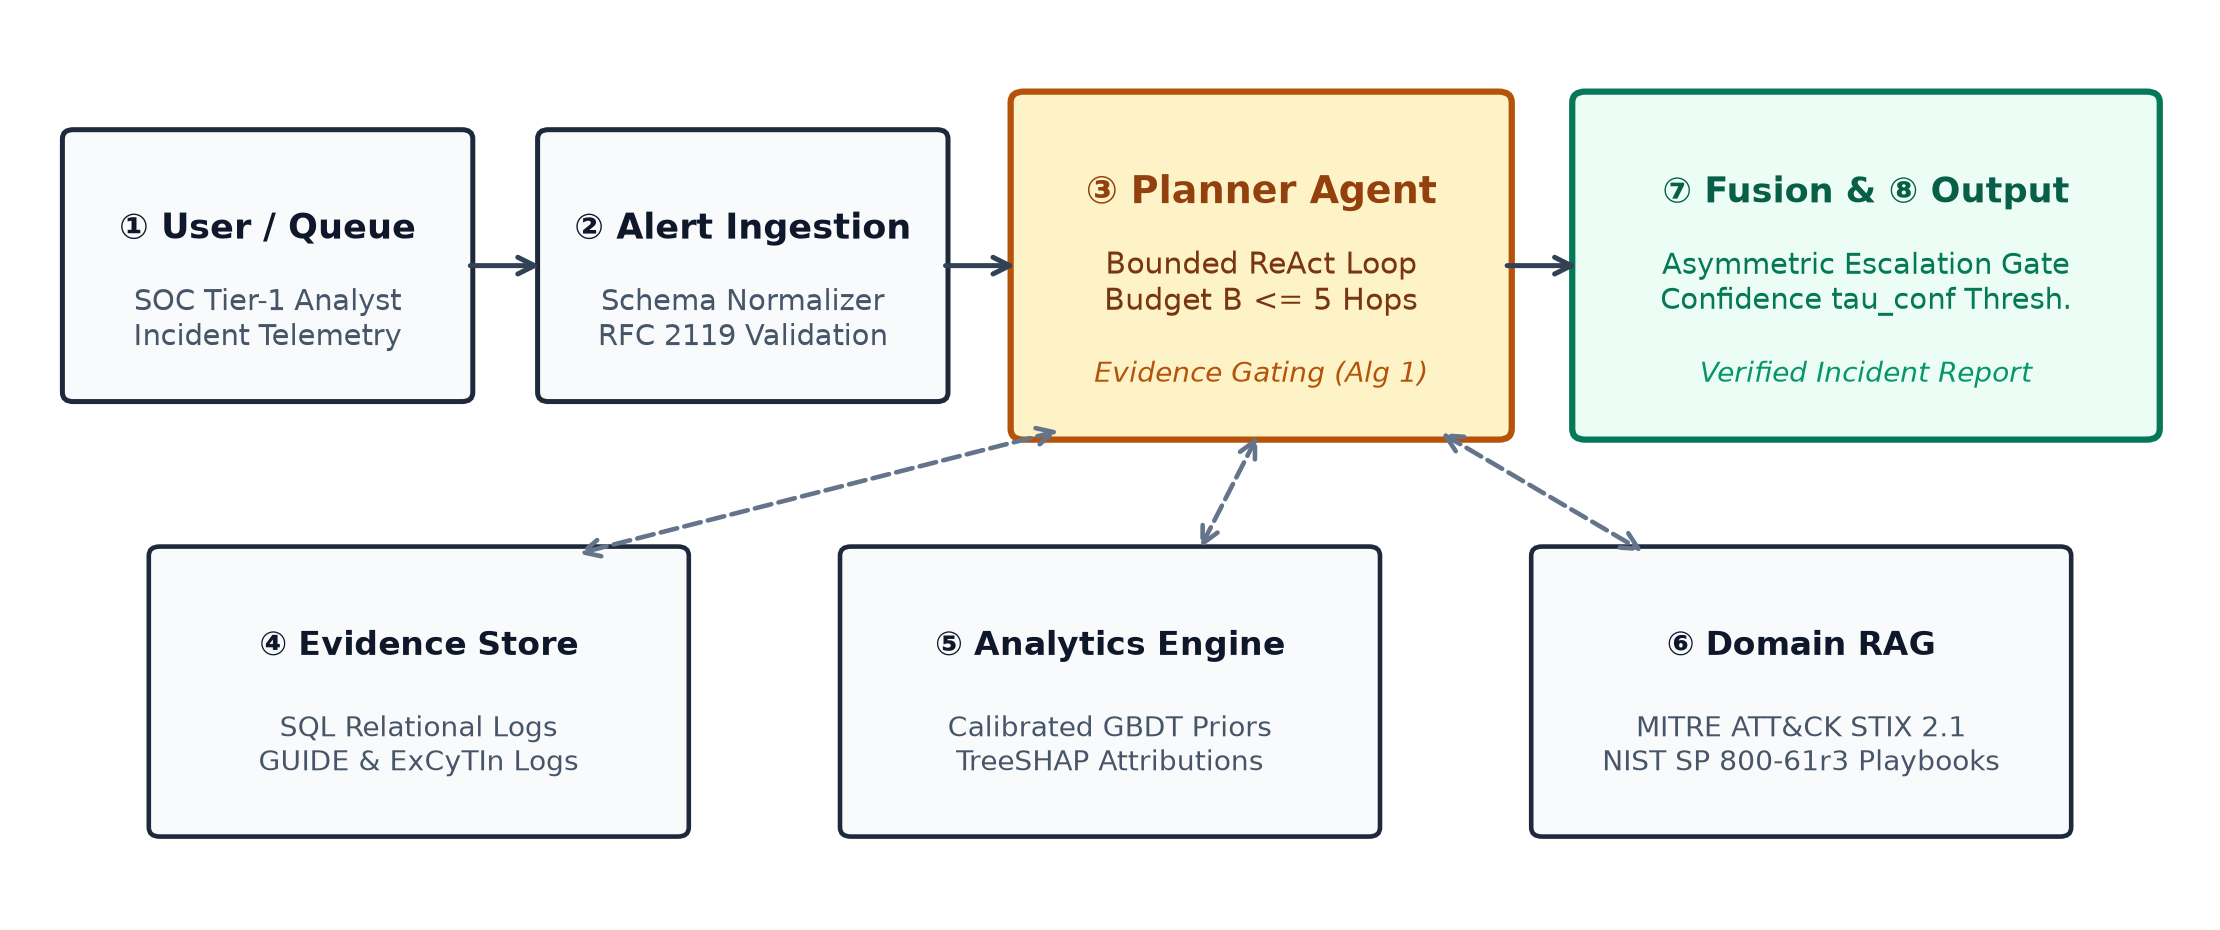
\includegraphics[width=\columnwidth]{fig1_architecture.png}
\caption{Eight-module functional architecture of the proposed AI SOC Analyst Agent.
Solid arrows denote data flow; the Evidence Gate enforces anti-premature-closure
invariants before the fusion verdict is issued.}
\label{fig:arch}
\end{figure}
